% % LLNCS macro package for Springer Computer Science proceedings;
% Version 2.21 of 2022/01/12
%
\documentclass[runningheads]{llncs}
%
\usepackage[T1]{fontenc}
% T1 fonts will be used to generate the final print and online PDFs,
% so please use T1 fonts in your manuscript whenever possible.
% Other font encondings may result in incorrect characters.
%
\usepackage{graphicx, color}
%
\usepackage{hyperref}
\renewcommand\UrlFont{\color{blue}\rmfamily}
\urlstyle{rm}
%

\begin{document}
    \title{MAFIA: An Adaptive Grid-Based Subspace Clustering Approach}
    %
    % Use \titlerunning{Abbreviated paper title}, if title is too long for the running head. Here, we can set an abbreviated paper title.
    %
    \author{Henrik Daniel Christensen\orcidID{hench13@student.sdu.dk}}
    \authorrunning{H. D. Christensen} % first names are abbreviated in the running head.
    %
    \institute{University of Southern Denmark, SDU\\\textit{Department of Mathematics and Computer Science}}
    %
    \maketitle % typeset the header of the contribution
    
    %%%%%%%%%%%%%%%%%%%%%%%%%%%%%%%%%%%%%%%%%%%
    \begin{abstract}
    This paper presents a comprehensive analysis of three bottom-up subspace clustering algorithms: \textit{MAFIA}, \textit{CLIQUE}, and \textit{SUBCLU}. MAFIA extends the grid-based approach of CLIQUE by introducing adaptive grid sizes, offering improved scalability and clustering quality. SUBCLU, in contrast, utilizes a density-connectivity method that allows better identification of arbitrarily shaped clusters, overcoming some of the limitations inherent in grid-based algorithms. The paper explores the relationships and distinctions between these algorithms, evaluating their performance in terms of scalability of dataset size, data- and cluster-dimensionality, as well as their clustering quality. Through a series of experiments with both synthetic and real-world datasets, we demonstrate the strengths and limitations of each approach. The findings reveal that while MAFIA is the most scalable, SUBCLU excels at detecting clusters with irregular shapes. However, all algorithms require proper parameter tuning for optimal performance.
    
    \keywords{High-Dimensional Subspace Clustering \and Grid-Based- and Density-Connectivity approach \and Comparative Study.}
\end{abstract}             % 0.4
    \section{Introduction}
\textit{Clustering} is one of the main techniques within data mining. The main goal is to discover unknown patterns within a data set, by partitioning the data objects into \textit{clusters}. Here, each object in a cluster is similar to one another, but different from objects in other clusters. Clustering is widely used in many applications, such as advertising, biology, web search and business intelligence \cite[p.~444]{han-2011}.

The task of clustering data is a challenging task, first, the data sets are typical large in size, which means that the clustering algorithm must be \textit{scalable}. Additionally, data sets often contains numerous features (\textit{attributes}), which introduces the problem of \textit{curse of dimensionality}, which refers to a several challenges related to high-dimensional data spaces:

First, the issue of \textit{concentration of distances}, where distances between objects in high-dimensional spaces become increasingly similar as dimensionality increases. This means that data points tend to become nearly equidistant from one another, making it difficult for traditional distance-based algorithms to discover clusters.

Secondly, there is the problem of \textit{local feature relevance} and \textit{local feature correlation}, where only a subset of features or different combinations of feature correlations may be relevant for clustering. Consequently, feature reduction techniques like \textit{Principal Component Analysis} (PCA), which project the original space onto a lower-dimensional subspace, are inadequate because they typically identify only one global subspace that best fits the entire dataset. Also, algorithms that evaluate the entire feature space does not address this issue effectively. \cite[p.~43--46]{kriegel-2009}

Instead of relying on a global approach to feature selection, a local approach that addresses the issues of local feature relevance and local feature correlation is necessary. However, we then need to deal with two separate problems, which both needs to be solved simultaneously. First, is the problem of finding the relevant subspaces of each cluster. Second, is the problem of finding the clusters in each relevant subspace. To solve them efficiently, heuristics needs to be employed into the clustering algorithms. \cite[p.~6--7]{kriegel-2009}

For many applications, it is reasonable to focus only on clusters in axis-parallel subspaces, thus restricting the search space to $O(2^d)$ dimensions. These algorithms are called \textit{subspace clustering} (or \textit{projected clustering}) algorithms. These can be further divided into: \textit{top-down}- or \textit{bottom-up} approach. In top-down approach, the relevant subspaces for the clusters are determined by gradually reducing the subspaces, starting from the entire space. In contrast, bottom-up approaches, finds the relevant subspaces for the clusters from the original space starting from 1-dimensional using the \textit{monotonicity property} (or \textit{downward closure property}), see Lemma \ref{lem:mono} \cite{clique}. \cite[p.~8,~11]{kriegel-2009}

For the rest of this paper, the following notation will be adopted: Let $\mathcal{A} = \{A_1, \dots, A_d\}$ represent the set of dimensions (attributes) in a $d$-dimensional numerical space, $\mathcal{S} = A_1 \times A_2 \times \dots \times A_d$. A subset of $\mathcal{A}$ is called a subspace. Let $\mathcal{D} = \{p_1, \dots, p_n\}$ be the dataset, where $p_i \in \mathcal{S}$ represents a data point. A cluster $\mathcal{C}$ is a subset of $\mathcal{D}$, where each point $p_i \in \mathcal{C}$ is more similar to the other points in $\mathcal{C}$ than to points outside of $\mathcal{C}$.

\begin{lemma}\label{lem:mono}
    If $\mathcal{C}$ is a cluster in a $k$-dimensional subspace, then $\mathcal{C}$ must also form a cluster in any $(k-1)$-dimensional projection of the same space.
\end{lemma}
A proof is provided in \cite{clique}.

\subsection{Contributions}
The primary focus of this paper is to analyze the grid-based bottom-up subspace clustering algorithm \textit{MAFIA} \cite{mafia}, which builds upon the first grid-based approach \textit{CLIQUE} \cite{clique}. This paper examines the relationship between these two, highlighting their similarities and differences. Additionally, the density-connectivity-based algorithm \textit{SUBCLU} \cite{subclu} is included, as it offers a contrasting approach to the grid-based approach.

The remainder of the paper is structured as follows: Section 2 describes and analyzes the three algorithms in detail. Section 3 evaluates their performance in terms of scalability, considering dataset size, data- and cluster-dimensionality, as well as their clustering quality. Section 5 discusses the findings and explores the contributions of each algorithm to the field of subspace clustering. Finally, Section 6 concludes the main findings and suggests some future work.         % 1
    \section{Subspace Clustering Algorithms}

\subsection{Grid-based approach}
Description of CLIQUE and briefly introduce how MAFIA extends it.

\subsection{Density-based approach}
Description of SUBCLU and describe how it relates to DBSCAN.  % 2
    \section{MAFIA}
\subsection{Adaptive Grids}

\subsection{MAFIA Algorithm}
- Simplified version of algorithm

\subsection{Candidate Dense Units (CDUs)}
- Why "any" dense unit                % 2
    \section{Evaluation}
The evaluation of the clustering algorithms was performed on a Intel i7 1.70 GHz processor (12th gen.) with 16 GB of RAM running Windows 11.

The evaluation of MAFIA was performed using \textit{GPUMAFIA} \cite{gpumafia}, which was installed on a virtual machine (VM) running Ubuntu 24.04.1 LTS using VirtualBox. The VM was configured with 4 CPUs and 4 GB of RAM.

In contrast, CLIQUE and SUBCLU were evaluated on the main machine using ELKI \cite{elki}. Thus, one should be careful to compare the results of the three algorithms directly, as the execution environment and the implementation may affect the results. However, the growth rate and the clustering quality of the algorithms can be compared.

Throughout the evaluation, a range of input parameters for the three algorithms were tested in the different experiments, where the best found parameters were selected. The evaluation project can be found in the GitHub repository: \url{https://github.com/henrikdchristensen/SDU-Data-Mining-Exam}. Here, also additional tests as well as detailed descriptions of how to generate the data sets and how to install and use GPUMAFIA can be found.

\subsection{Data set generation}
The aim for the synthetic data generation was to be able to produce similar data sets as discussed in \cite{mafia}. That is, data sets containing axis-parallel clusters in different subspaces, clusters with different sizes and different densities. This was achieved by using \textit{MDCGen} that could create large high-dimensional axis-parallel clustered data sets. Furthermore, it was possible to determine for each cluster which of the attributes that are noise, in which values at random from a uniform distribution over the entire range of the attribute were selected.

However, to see the one of the main advantages of SUBCLU compared to CLIQUE and MAFIA, a data set containing a Bezier-shaped cluster was created using \textit{Artificial Cluster} (AC). In addition, a self-populated data set containing a plus-shaped cluster was created as discussed in \cite{mafia}.

Finally, two real-world data sets were selected to evaluate the algorithms in a more realistic setting.

All the data sets were normalized such that each attribute was in the range [0, 1].

\subsection{Experimental Results}

\subsubsection{Scalability with Data Set Size}
To evaluate the scalability of the algorithms a data set containing 20 dimensions with 5 clusters in 5 different subspaces with 10\% noise records was used. The data set size ranges from 10k to 1mio records. The results can be seen in Figure \ref{fig:dataset_size_vs_runtime}. As can be seen, MAFIA is the most scalable algorithm of the three. CLIQUE could handle up to 500k records, while SUBCLU was only able to handle up to 100k records. Similar results were reported in all three papers \cite{mafia,clique,subclu}. However, the non-linear grow of SUBCLU after 20k records reported in \cite{subclu} happens first after 100k records in this experiment. Moreover, to achieve this growth rate of SUBCLU, we had to scale the minpts linearly with the data set size, this is due to the fact that the dateset contains clusters having a fixed size and by increasing the data set size, the density of the clusters increases linearly. However, for the other two algorithms, there was no need to scale the input parameters, as they relies on the grids.
\begin{figure}[H]
    \vspace*{-0.5cm}
    \centering
    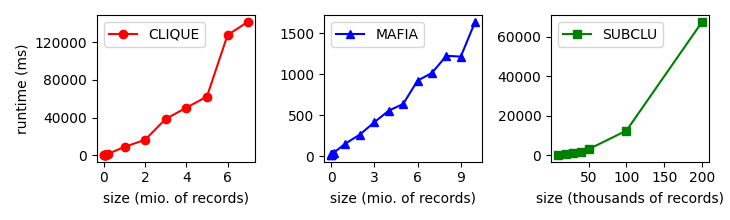
\includegraphics[scale=0.45]{figures/dataset_size_vs_runtime.png}
    \caption{Scalability with increasing data set size.}
    \label{fig:dataset_size_vs_runtime}
    \vspace*{-0.5cm}
\end{figure}

\subsubsection{Clustering Accuracy}
Many different synthetic data sets were generated to test the clustering accuracy of the algorithms.

The first data set were a 2-dimensional data set containing a single cluster formed as a plus with 10\% noise added, as discussed in \cite{mafia}. MAFIA, was able to detect the 2-dimensional cluster almost completely, whereas CLIQUE only partly detects the cluster and the clusters overlaps. The accuracy of MAFIA comes however with a cost, as it also reports some lower-dimensional clusters as well. The results can be seen in Figure \ref{fig:accuracy_plus}. The effect of adaptive grid sizes, clearly shows that MAFIA is more flexible than CLIQUE in such cases.
\begin{figure}[H]
    \vspace*{-0.5cm}
    \centering
    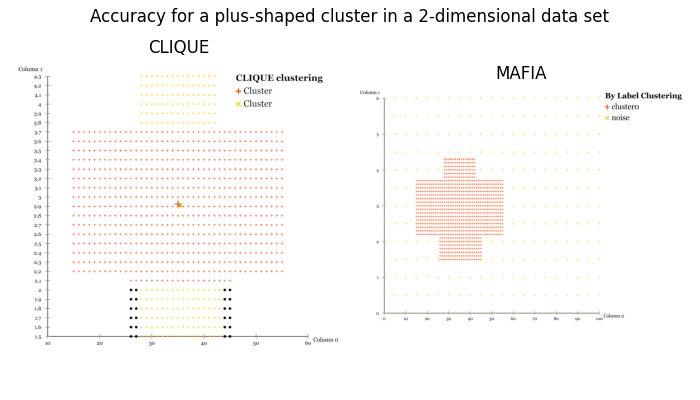
\includegraphics[scale=0.27]{figures/accuracy_plus.png}
    \caption{A single plus-shaped cluster.}
    \label{fig:accuracy_plus}
    \vspace*{-0.5cm}
\end{figure}

The second data set contains 10 dimensions with contains 2 clusters embedded in a different 4 dimensional subspace. 10\% of the data was added as noise records. Similar data set as the one used in \cite{mafia}. The results can be seen in Figure \ref{fig:accuracy_2clusters}. Here, MAFIA was able to detect the clusters without any additional lower-dimensional clusters. In contrast, CLIQUE reports some overlapping clusters and some of the noise records as clusters. SUBCLU detects also the two clusters, but reports many lower-dimensional clusters and noise records as clusters as well.
\begin{figure}[H]
    \vspace*{-0.5cm}
    \centering
    \subfloat[][CLIQUE]{%
        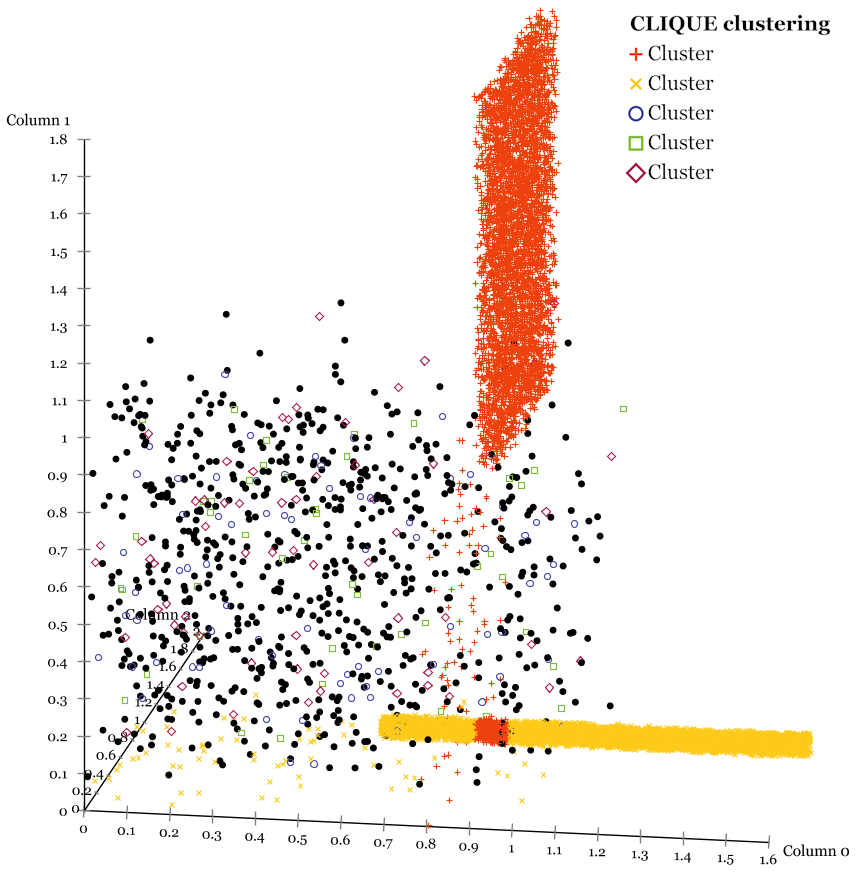
\includegraphics[width=0.3\textwidth]{figures/accuracy_2clusters/clique.png}\label{fig:accuracy_2clusters_clique}}~~~~
    \subfloat[][MAFIA]{%
        \includegraphics[width=0.3\textwidth]{figures/accuracy_2clusters/MAFIA.png}\label{fig:accuracy_2clusters_mafia}}~~~~
    \subfloat[][SUBCLU]{%
        \includegraphics[width=0.3\textwidth]{figures/accuracy_2clusters/SUBCLU.png}\label{fig:accuracy_2clusters_subclu}}
    \caption{Two clusters in 4 different subspaces.}
    \label{fig:accuracy_2clusters}
    \vspace*{-0.5cm}
\end{figure}

The third data set were a 2-dimensional data set containing a single cluster formed as a Bezier curve with 10\% noise added to the data set. As expected, SUBCLU outperforms the other two algorithms as can be seen in Figure \ref{fig:accuracy_bezier}. MAFIA and CLIQUE only partly detects the cluster and reports additional clusters and noise records as clusters. The result of SUBCLU demonstrates its locality assumption and its use of DBSCAN.
\begin{figure}[H]
    \vspace*{-0.5cm}
    \centering
    \subfloat[][CLIQUE]{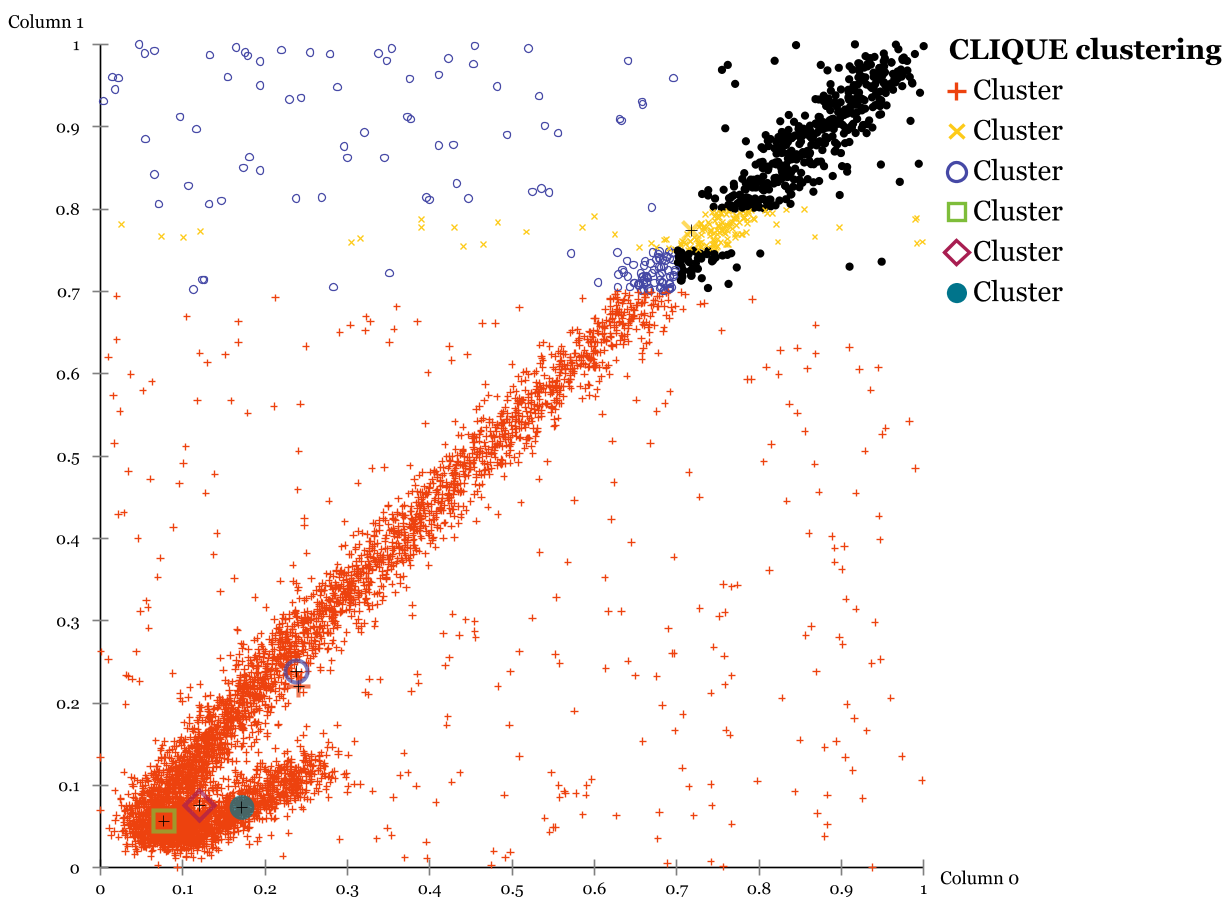
\includegraphics[width=0.3\textwidth]{figures/accuracy_bezier/clique.png}\label{fig:accuracy_bezier_clique}}~~~~
    \subfloat[][MAFIA]{\includegraphics[width=0.3\textwidth]{figures/accuracy_bezier/MAFIA.png}\label{fig:accuracy_bezier_mafia}}~~~~
    \subfloat[][SUBCLU]{\includegraphics[width=0.3\textwidth]{figures/accuracy_bezier/SUBCLU.png}\label{fig:accuracy_bezier_subclu}}
    \caption{A single bezier-shaped cluster.}
    \label{fig:accuracy_bezier}
\end{figure}

\subsubsection{Scalability with Data Dimensionality and Cluster Dimensionality}
Figure \ref{fig:data_dimensionality_vs_runtime} shows the scalability of the CLIQUE and MAFIA with increasing data set dimensionality. The data set contains 1 mio. records with 3 clusters in 5 different subspaces and 10\% noise records, similar to the data set in \cite{mafia}. The data set dimensionality ranges from 10 to 100 dimensions. The results clearly shows that MAFIA is the most scalable algorithm.
\begin{figure}[H]
    \vspace*{-0.5cm}
    \centering
    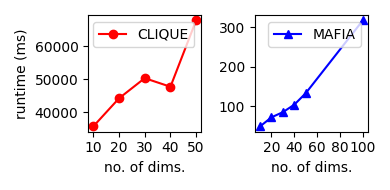
\includegraphics[scale=0.45]{figures/data_dimensionality_vs_runtime.png}
    \caption{Scalability with increasing data set dimensionality.}
    \label{fig:data_dimensionality_vs_runtime}
    \vspace*{-0.5cm}
\end{figure}

Figure \ref{fig:cluster_dimensionality_vs_runtime} shows the scalability of the CLIQUE and MAFIA with increasing cluster dimensionality. The data set contains 500k records with one single cluster. The cluster was embeeded in increasing number of dimensions starting from 10 to 100 dimensions. 10\% of the records was added as noise The data set contains in total 20 dimensions. The data set is similar to the one used in \cite{mafia}. The results clearly shows that MAFIA is the most scalable algorithm of the two.
\begin{figure}[H]
    \vspace*{-0.5cm}
    \centering
    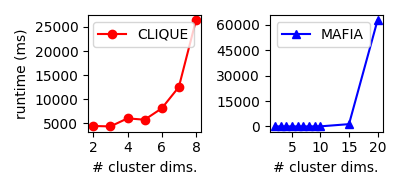
\includegraphics[scale=0.45]{figures/cluster_dimensionality_vs_runtime.png}
    \caption{Scalability with increasing cluster dimensionality.}
    \label{fig:cluster_dimensionality_vs_runtime}
    \vspace*{-0.5cm}
\end{figure}

The results reported for SUBCLU in \cite{subclu} were also tried to be replicated, however, similar it was not possible evaluate in different scales of data set dimensionality and cluster dimensionality, as the PC constantly freezes -- probably due to the high memory consumption. In future work, it would be interesting to investigate this further.

\subsection{Sensitive analysis for MAFIA}
According to \cite{mafia}, MAFIA should not be sensitive to the choice of $\alpha$. A 20-dimensional data set with 1mio data points with 10\% noise was used to evaluate this. $\beta$ was fixed to 35\%, and $\alpha$ was ranging from 0.8 to 5.2 in step size of 0.4. The results can be seen in Figure \ref{fig:sensitivity_alpha}. From the results one could again draw the conclusion that MAFIA is not very sensitive to the $\alpha$ parameter. However, during evaluation of different types of data sets, many different values $\alpha$ was used to detect the right clusters. Also, different $\beta$ values as well as maximum number of windows was needed to be set properly to achieve meaningful results.
\begin{figure}[H]
    \vspace*{-0.5cm}
    \centering
    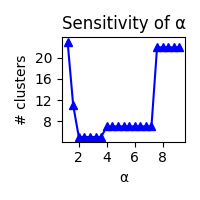
\includegraphics[scale=0.45]{figures/sensitivity_alpha.png}
    \caption{Sensitivity of $\alpha$ for MAFIA.}
    \label{fig:sensitivity_alpha}
\end{figure}

\subsubsection{Real Data Sets}
Two real-world data sets are used to evaluate the algorithms in a more realistic setting. Small data sets were selected for both performance and visualization reasons. Both data sets were normalized such that each attribute was in the range [0, 1].

The first data set is the well-known \textit{Iris} data set \cite{iris}, which contains 150 records of 3 different iris types (e.g. Setosa, Versicolor, Virginica). The data set contains 4 features (sepal length, sepal width, petal length and petal width). All three algorithms produced some meaningful clusters, however, as can be seen in Figure \ref{fig:real_world_iris}. It is hard to determine which algorithm performs the best in this case.
\begin{figure}[H]
    \vspace*{-0.5cm}
    \centering
    \subfloat[][Original]{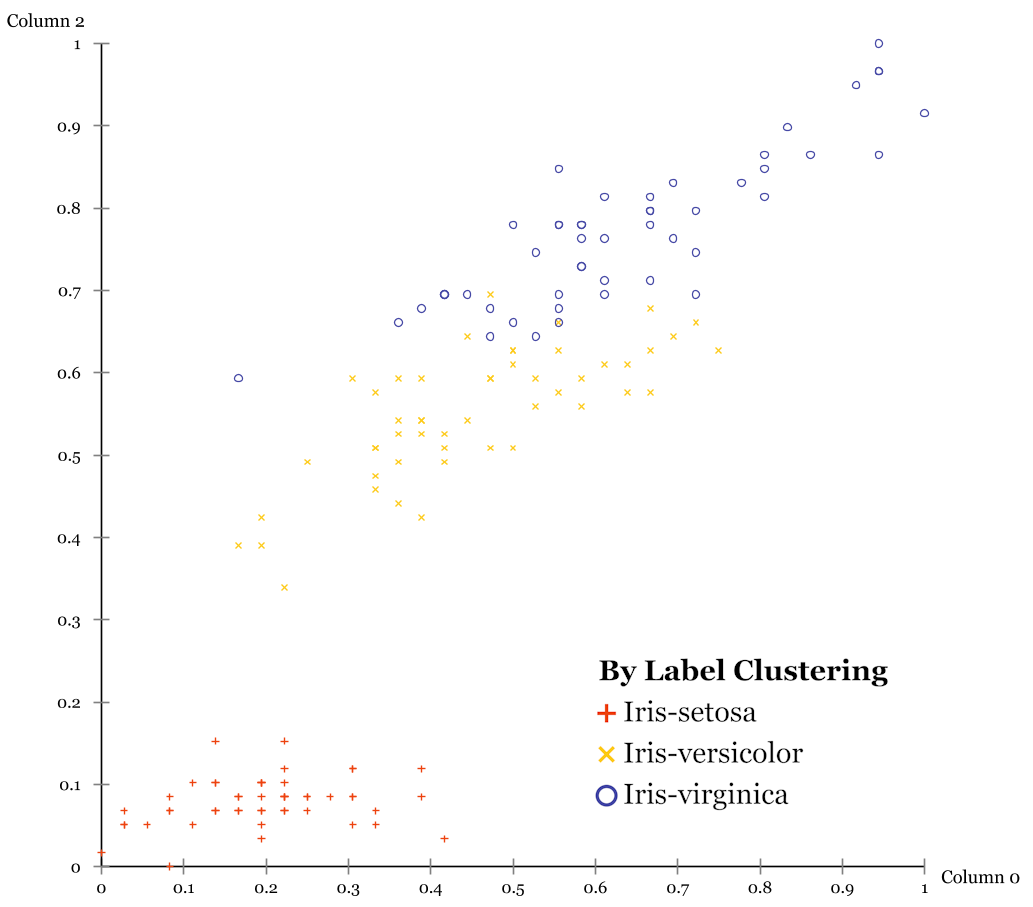
\includegraphics[width=0.25\textwidth]{figures/real_world_iris/orig.png}\label{fig:real_world_iris_orig}}~~~~
    \subfloat[][CLIQUE]{\includegraphics[width=0.25\textwidth]{figures/real_world_iris/CLIQUE.png}\label{fig:real_world_iris_clique}}\\
    \subfloat[][MAFIA]{\includegraphics[width=0.25\textwidth]{figures/real_world_iris/MAFIA.png}\label{fig:real_world_iris_mafia}}~~~~
    \subfloat[][SUBCLU]{\includegraphics[width=0.25\textwidth]{figures/real_world_iris/SUBCLU.png}\label{fig:real_world_iris_subclu}}
    \caption{Iris data set.}
    \label{fig:real_world_iris}
    \vspace*{-0.5cm}
\end{figure}

The second data set is the \textit{Date Fruit} data set \cite{date-fruit}, which contains 898 records of 7 different date fruit types (e.g. Barhee, Deglet Nour, Sukkary, Rotab). These were obtained via a computer vision, where 34 features (e.g shape and color) was extracted. Only SUBCLU were able to produce meaningful results, see Figure \ref{fig:real_world_date_fruit}. CLIQUE and MAFIA either produced way too many clusters or close to one single cluster.
\begin{figure}[H]
    \vspace*{-0.5cm}
    \centering
    \subfloat[][Original]{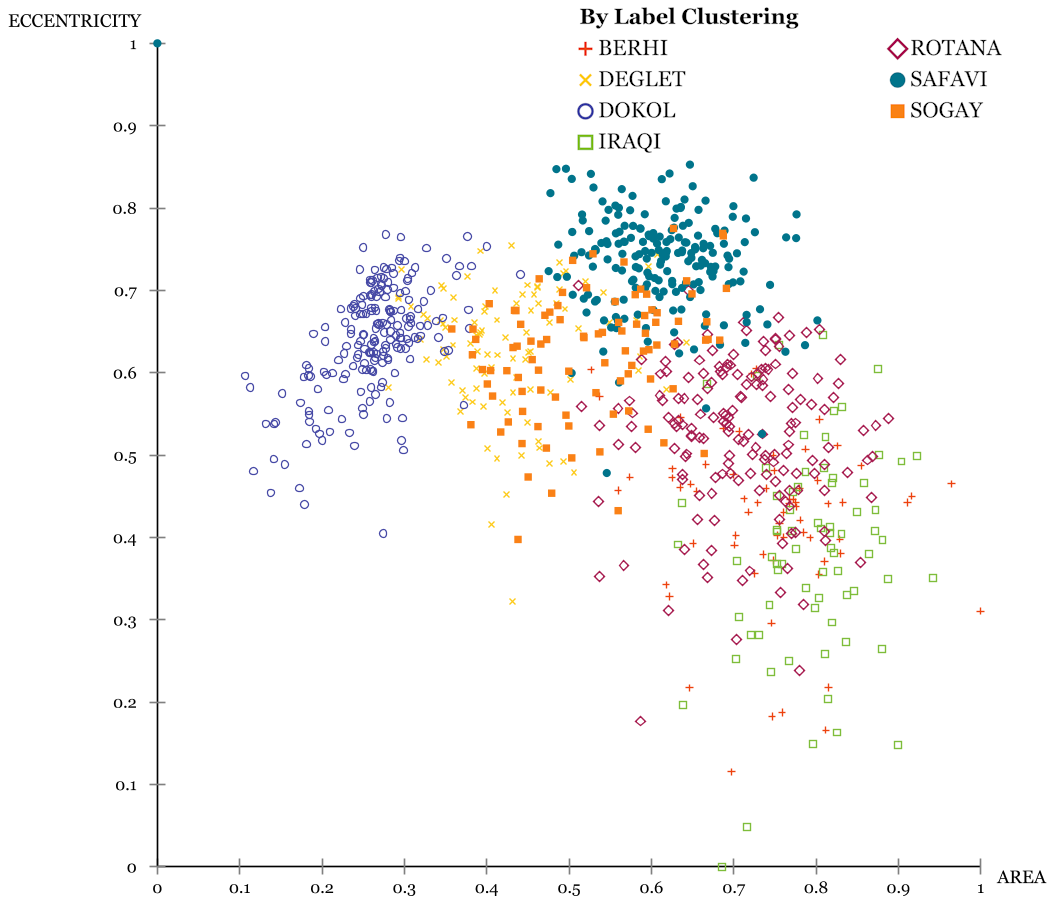
\includegraphics[width=0.25\textwidth]{figures/real_world_date_fruit/orig.png}\label{fig:real_world_date_fruit_orig}}~~~~
    \subfloat[][SUBCLU]{\includegraphics[width=0.25\textwidth]{figures/real_world_date_fruit/SUBCLU.png}\label{fig:real_world_date_fruit_subclu}}
    \caption{Date Fruit data set.}
    \label{fig:real_world_date_fruit}
\end{figure}           % 3
    \section{Discussion}
\begin{itemize}
    \item Discussion of the different approaches
    \item Discussion of results
    \item Limitations and Strengths
    \item Model: Input parameters; Assumptions on number, size, and shape of clusters; Noise
    \item Determinism
    \item Independence w.r.t. order of objects/attributes
    \item Assumptions on overlap/non-overlap of clusters/subspaces
    \item Effiency
\end{itemize}


Interpretability and usability: Clustering results should be easy to interpret and algorithms should produce clusters that are meaningful and comprehensible, making the results practical for decision-making.

Discovery of arbitrary-shaped clusters: Many clustering algorithms are limited to detecting spherical clusters based on distance measures (e.g. Euclidean distance). However, clusters in real-world data often take arbitrary shapes.

Minimize dependence on domain knowledge: Many clustering algorithms require users to provide specific input parameters, such as the number of clusters, which can be challenging to determine a prior. Reducing such parameters not only simplifies the process for users but also improve the reliability of the results.

Robust to noisy data: Real-world data is often noisy or contains outliers, which can distort clustering results. Clustering algorithms should be robust enough to handle noisy data, missing values, and outliers without degrading the quality of the clusters.

\cite[p.~446-447]{han-2011}           % 3
    \section{Conclusion}
Main findings           % 0.5
    %%%%%%%%%%%%%%%%%%%%%%%%%%%%%%%%%%%%%%%%%%%
    
    %%%%%%%%%%%%%%%%%%%%%%%%%%%%%%%%%%%%%%%%%%%
    %\begin{credits}
    \subsubsection{\ackname}
    A bold run-in heading in small font size at the end of the paper is
    used for general acknowledgments, for example: This study was funded
    by X (grant number Y).
    
    \subsubsection{\discintname}
    It is now necessary to declare any competing interests or to specifically
    state that the authors have no competing interests. Please place the
    statement with a bold run-in heading in small font size beneath the
    (optional) acknowledgments\footnote{If EquinOCS, our proceedings submission
    system, is used, then the disclaimer can be provided directly in the system.},
    for example: The authors have no competing interests to declare that are
    relevant to the content of this article. Or: Author A has received research
    grants from Company W. Author B has received a speaker honorarium from
    Company X and owns stock in Company Y. Author C is a member of committee Z.
\end{credits}
    
    
    \bibliographystyle{base/splncs04}
    \bibliography{base/references}
    %%%%%%%%%%%%%%%%%%%%%%%%%%%%%%%%%%%%%%%%%%%
\end{document}